\documentclass[12pt,]{article}
\usepackage[utf8]{inputenc}
\usepackage[T1]{fontenc}
\usepackage{mathptmx}
\usepackage{geometry}
\usepackage{mathtools}
\usepackage[english]{babel}
\usepackage{graphicx}
\usepackage[os=win]{menukeys}
\usepackage[figurename=Gambar]{caption}
\usepackage{hyperref}
\usepackage{minted}
\usepackage{float}
\usepackage{pdflscape}
\usepackage{pdfpages}
\usepackage{tikz}


\addto\captionsenglish{\renewcommand{\contentsname}{Daftar Isi}}
\addto\captionsenglish{\renewcommand{\bibname}{Referensi}}

\hypersetup{
	colorlinks=true, %set true if you want colored links
	linktoc=all,     %set to all if you want both sections and subsections linked
	linkcolor=blue,  %choose some color if you want links to stand out
}

\geometry{
	a4paper,
	left=15mm,
	right=10mm,
	top=10mm,
	bottom=10mm,
}

\usetikzlibrary{positioning}
\tikzstyle{squared} = [rectangle, rounded corners, minimum width=1cm, minimum height=0.5cm,text centered, draw=black]
\tikzstyle{connect} = [ultra thick,->]
\tikzstyle{connect2} = [ultra thick,<->]

\title{\Large \bf
	Pengenalan GNU/Linux dan Lingkungan Pemrogramannya.
}

\author{Achmadi ST s.MT}
\date{}

\begin{document}
	\maketitle
	\thispagestyle{empty}
	\pagestyle{empty}
	
	\newpage
	\tableofcontents
	
	\newpage
	\section{GNU/Linux}
	
	\subsection{Pengenalan}
	\hspace{10pt} Linux adalah \textit{kernel} sistem operasi komputer yang dibuat di tahun 1991 oleh mahasiswa Finlandia, Linus Benedict Torvald.
	Linux dirancang sangat mirip dengan kernel sistem operasi UNIX yang dibuat oleh lab AT\&T (semacam Telkom di USA).
	Selain Linux, kernel lain yang juga berbasis UNIX antara lain Darwin (MacOS) dan BSD (Berkeley OS).
	
	Kernel adalah bagian terpenting dari sistem operasi.
	Kernel memiliki tugas antara lain:
	\begin{itemize}
		\item Mengatur alokasi memori (RAM) dan processor ()CPU)
		\item Mengatur permintaan layanan/sumber daya hardware dan software
	\end{itemize}
	
	Untuk membentuk sistem operasi yang bisa dipakai, kernel saja tidak cukup.
	Dibutuhkan sistem antar-muka (\textit{interface}) dan software alat bantu (\textit{tools}).
	Disinilah peran GNU. 
	GNU adalah organisasi yang dibentuk oleh Richard Stallman.
	Karya GNU antara lain software interface/tools, translasi, dan dokumentasi.
	Dan karya terbesar GNU adalah membuat lisensi \textit{open-sources} memiliki kekuatan hukum.
	
	Open-source adalah bentuk/model pengembangan software dimana pengembang memberikan hak akses kode sumber (\textit{source-code}) kepada pengguna.
	Open-source memberikan hak kepada pengguna antara lain:
	\begin{itemize}
		\item Hak untuk menggandakan
		\item Hak untuk mempelajari
		\item Hak untuk memodifikasi
		\item Hak untuk menyebarluaskan
	\end{itemize}
	Dalam proses memberikan akses kode sumber, pengembang dapat memberikan hak akses secara berbayar atau bisa juga gratis.
	
	\subsection{Struktur}
	Secara sederhana, struktur sistem operasi GNU/Linux adalah sebagai berikut:
	\begin{figure}[H]
		\begin{center}
			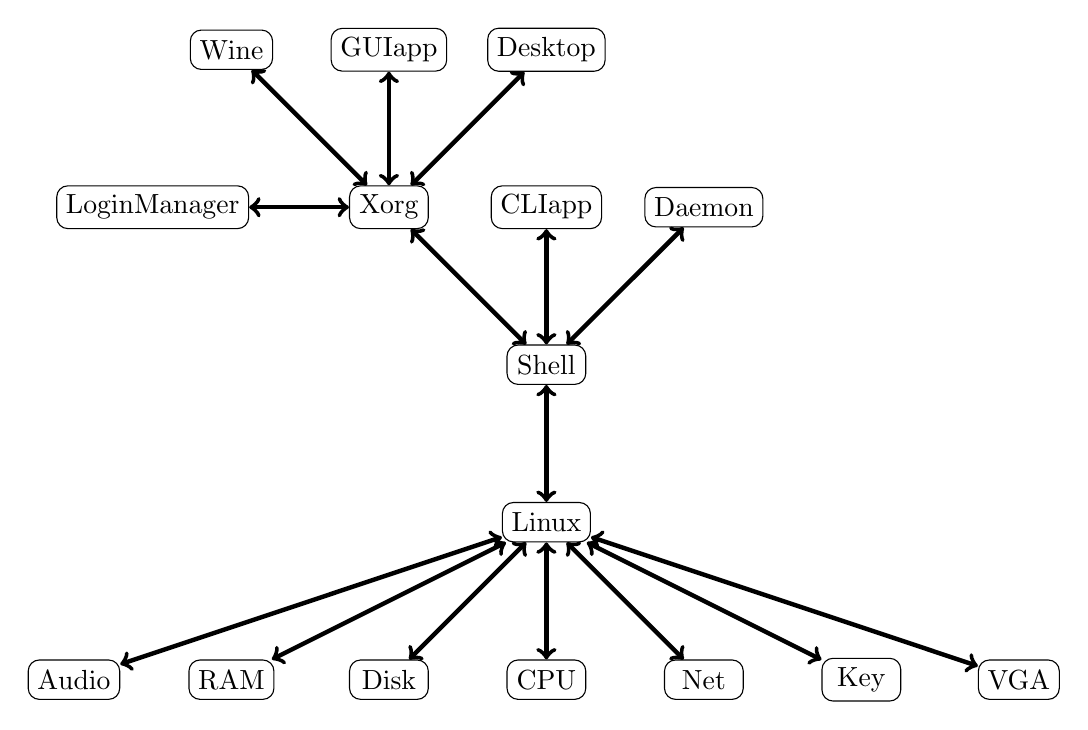
\begin{tikzpicture}[node distance=2cm]
			\node (linux) [squared] {Linux};
			\node (shell) [squared, above of=linux] {Shell};
			\node (cpu) [squared, below of=linux] {CPU};
			\node (ram) [squared, left of=cpu] {Disk};
			\node (disk) [squared, left of=ram] {RAM};
			\node (audio) [squared, left of=disk] {Audio};
			\node (net) [squared, right of=cpu] {Net};
			\node (key) [squared, right of=net] {Key};
			\node (vga) [squared, right of=key] {VGA};
			\node (cli) [squared, above of=shell] {CLIapp};
			\node (xorg) [squared, left of=cli] {Xorg};
			\node (gui) [squared, above of=xorg] {GUIapp};
			\node (login) [squared, left of=xorg,xshift=-1cm] {LoginManager};
			\node (de) [squared, right of=gui] {Desktop};
			\node (daemon) [squared, right of=cli] {Daemon};
			\node (wine) [squared, left of=gui] {Wine};
			
			\draw [connect2] (linux) -- (shell);
			\draw [connect2] (linux) -- (cpu);
			\draw [connect2] (linux) -- (ram);
			\draw [connect2] (linux) -- (disk);
			\draw [connect2] (linux) -- (audio);
			\draw [connect2] (linux) -- (net);
			\draw [connect2] (linux) -- (key);
			\draw [connect2] (linux) -- (vga);
			\draw [connect2] (shell) -- (cli);
			\draw [connect2] (shell) -- (xorg);
			\draw [connect2] (shell) -- (daemon);
			\draw [connect2] (xorg) -- (login);
			\draw [connect2] (xorg) -- (gui);
			\draw [connect2] (xorg) -- (de);
			\draw [connect2] (xorg) -- (wine);
			\end{tikzpicture}
			\caption{Diagram Struktur Sistem Operasi Linux}
		\end{center}
	\end{figure}

	\subsection{Distro GNU/Linux}
	Seperti yang dijelaskan sebelumnya, Linux sendiri tidak bisa sebagai sistem operasi.
	Bersama dengan Linux, ditambahkan beragam software sehingga membentuk sistem operasi lengkap.
	Paket lengkap ini dikenal sebagai distribusi atau distro GNU/Linux.
	Hari ini dikenal total ada 305 (hasil data yang terdaftar di \url{https://distrowatch.com/}).
	Beberapa yang terkenal antara lain:
	\begin{itemize}
		\item Ubuntu. Distro GNU/Linux yang dirilis oleh Canonical, perusahaan raksasa IT di UK.
		\item LinuxMint. Distro GNU/Linux turunan Ubuntu yang dirilis oleh Clement Lefebvre dan timnya.
		\item Fedora. Distro GNU/Linux yang dirilis oleh Red Hat,
		perusahaan raksasa IT yang berdiri 1993 dan merupakan salah satu perusahaan open-source terbesar di dunia.
		\item Debian. Distro GNU/Linux berbasis komunitas tertua. Ubuntu, LinuxMint, dan puluhan distro merupakan turunan dari Debian.
		\item Arch Linux. Distro GNU/Linux berbasis komunitas yang terkenal sebagai distro DIY (Do It Yourself).
	\end{itemize}
	
	Pada pelatihan ini, dipilih Arch Linux dengan alasan:
	\begin{itemize}
		\item Arch Linux menyerahkan sepenuhnya instalasi ke user.
		\item Paket yang terinstal bisa sesuai yang dibutuhkan. 
		\item Arch Linux memiliki cakupan repository sangat luas.
		Hampir semua bisa diinstal di platform Arch Linux.
		\item Halaman Wiki yang dimiliki Arch Linux adalah yang paling lengkap.
		\item Arch Linux berbasis rolling-release.
		Artinya bila perlu upgrade/update, tidak perlu instal ulang sistem operasi.
		\item Arch Linux tidak diatur oleh perusahaan manapun. 
		Benar-benar community-driven
		\item Arch Linux tergolong bleeding-edge. Repository update/upgrade dalam hitungan minggu.
		\item Arch Linux melatih pengguna dari sisi teknis secara detail.
	\end{itemize}

	\subsection{Persiapan VBox}
	Selanjutnya bagian praktikum, akan ditunjukkan langkah-langkah persiapan VirtualBox (VBox).
	VBox disini akan menjadi unit komputer virtual alat belajar.
	
	\subsubsection{Virtualbox}
	Virtualbox adalah software yang digunakan sebagai virtual komputer.
	Virtualbox dapat menjalankan sistem operasi layaknya komputer pada umumnya.
	Virtualbox memiliki perangkat bersifat virtual meliputi cpu, memory, harddisk, cd/dvd rom, ethernet card, dst
	Untuk menggunakan VirtualBox 64bit disini, syarat yang harus dipenuhi:
	\begin{itemize}
		\item CPU laptop anda mendukung 64bit (amd64, ia64, x86\_64) sistem
		\item Fitur Virtualisasi di CPU sudah diaktifkan (melalui BIOS/UEFI)
	\end{itemize}
	
	\subsubsection{Buat unit komputer baru}
	\begin{itemize}
		\item Download dan install VirtualBox di alamat situs: \url{https://www.virtualbox.org/wiki/Downloads}.
		Silahkan cek tutorial seperti:
		\begin{itemize}
			\item \url{https://www.smarthomebeginner.com/install-virtualbox-on-windows/}
			\item \url{https://siteblogforu.blogspot.com/2014/02/cara-install-virtualbox-di-windows-7.html}
			\item \url{http://www.duniacara.com/2018/03/cara-menginstall-virtualbox-di-windows-10}
		\end{itemize}
		\item Tekan tombol \textbf{New} dan pilih OS Linux (Arch Linux 64bit).
		Tekan tombol \textbf{Next}
		\begin{figure}[H]
			\centering
			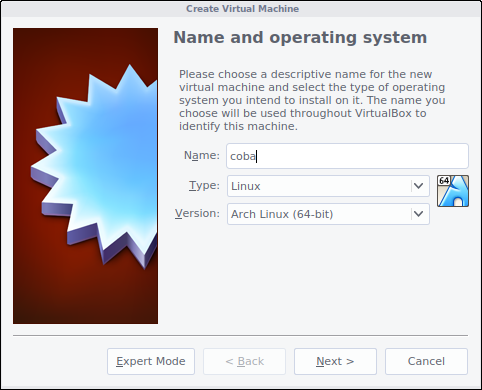
\includegraphics[width=0.4\linewidth]{images/vbox_installinux/s1}
			\caption{Pilih OS}
		\end{figure}
	
		\item Selanjutnya akan ada pengaturan RAM, isi minimal \textbf{1024}MB.
		Sesuaikan dengan RAM komputer yang tersedia.
		
		\item Selanjutnya akan ada pilihan membuat virtual Disk baru.
		Pilih \textbf{Create virtual hard disk now}.
		Tekan tombol \textbf{Create}
		
		\item Selanjutnya akan ada pilihan tipe virtual Hardisk.
		Pilih \textbf{VDI}. Tekan tombol \textbf{Next}
		
		\item Selanjutnya akan ada pilihan tipe alokasi.
		Pilih \textbf{Fixed Size}.
		Tekan tombol \textbf{Next}
		
		\item Selanjutnya akan ada pengaturan ukuran disk.
		Pilih ukuran 8GB. Sesuaikan dengan sisa ukuran di partisi hardisk komputer yg tersedia.
		Tekan tombol \textbf{Create}
		\begin{figure}[H]
			\centering
			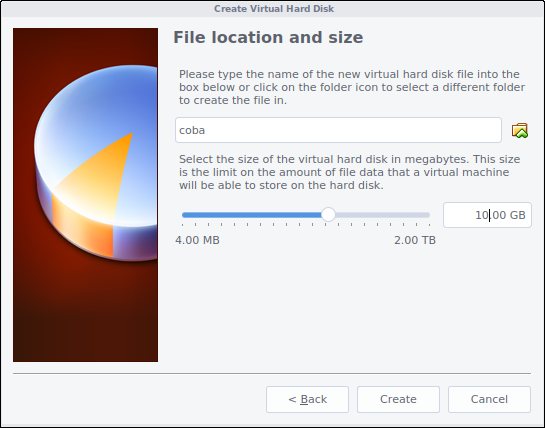
\includegraphics[width=0.4\linewidth]{images/vbox_installinux/s2}
			\caption{Virtual Disk}
		\end{figure}
	\end{itemize}
	
	\subsubsection{Pasang DVD/ISO Instalasi}
	\begin{itemize}
		\item Selanjutnya tekan tombol \textbf{Settings}. Pilih tab \textbf{Storage}.
		\begin{figure}[H]
			\centering
			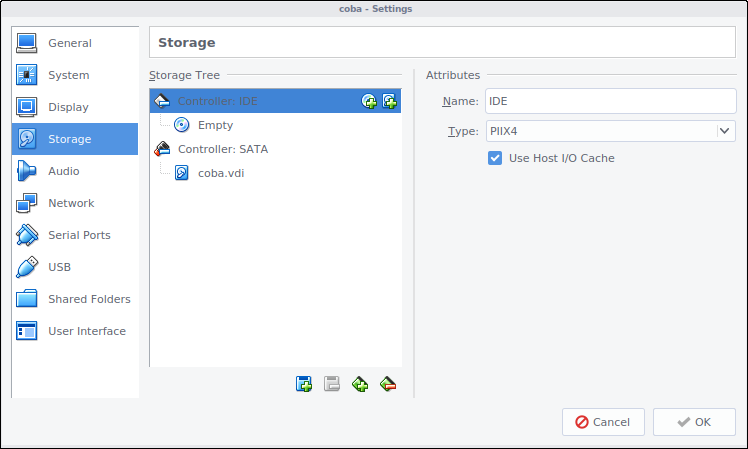
\includegraphics[width=0.4\linewidth]{images/vbox_installinux/s3}
			\caption{Pilih iso instalasi}
		\end{figure}
	
		\item Pada bagian CD/DVD, isi file iso koleksi paket.
		ISO yang digunakan adalah \textit{archlinuxpkg\_2015.iso}.
		Jika belum mendapatkan silahkan minta trainer.
		\begin{figure}[H]
			\centering
			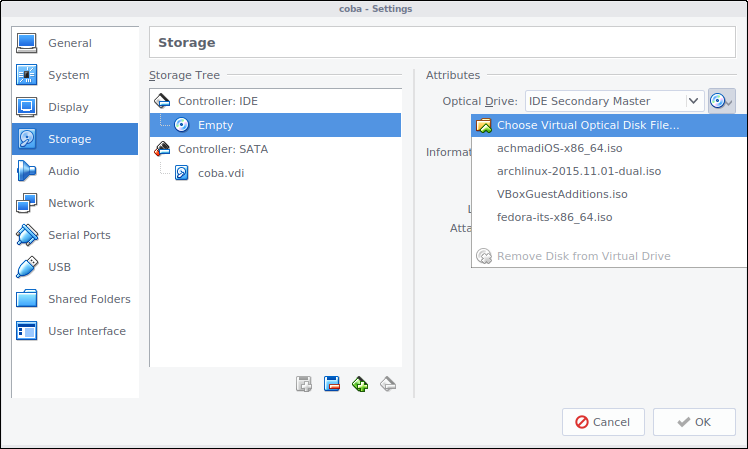
\includegraphics[width=0.4\linewidth]{images/vbox_installinux/s4}
			\caption{Pilih iso paket}
		\end{figure}
	
		\item Pilih mode drive ISO terakhir menjadi \textbf{IDE Primary Slave}.
		\begin{figure}[H]
			\centering
			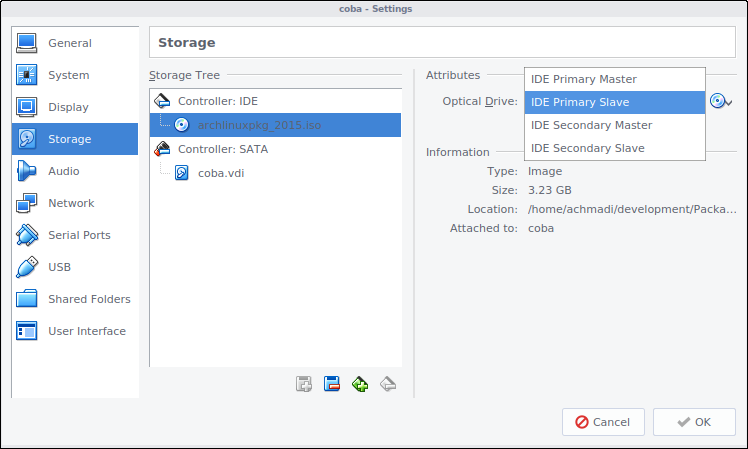
\includegraphics[width=0.4\linewidth]{images/vbox_installinux/s5}
			\caption{iso paket terpasang}
		\end{figure}
	
		\item Langkah terakhir adalah memasang iso instalasi.
		ISO yang digunakan adalah \textit{archlinux-2015.11.01-dual.iso}.
		Jika belum mendapatkan silahkan minta trainer.
		Tekan icon \textbf{Add Optical Drive}.
		Selanjutnya pilih Choose Disc.
		\begin{figure}[H]
			\centering
			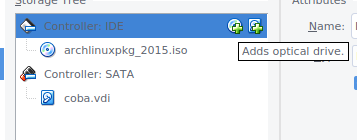
\includegraphics[width=0.4\linewidth]{images/vbox_installinux/s6}
			\caption{tombol tambah Optical Drive}
		\end{figure}
	
		\item Pilih mode drive ISO terakhir menjadi \textbf{IDE Primary Master}.
		\begin{figure}[H]
			\centering
			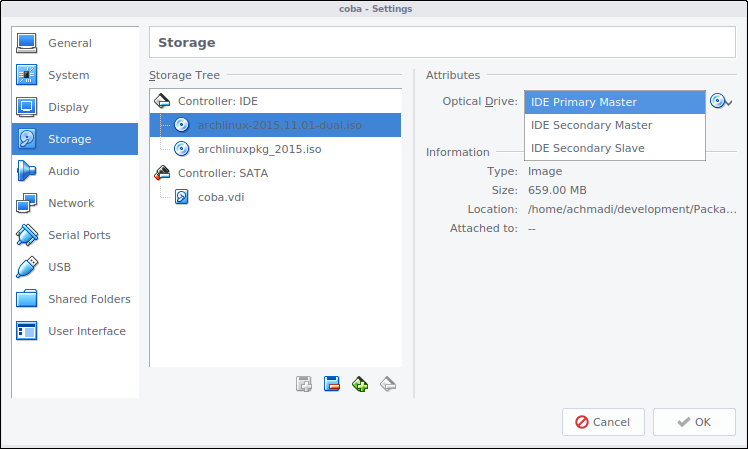
\includegraphics[width=0.4\linewidth]{images/vbox_installinux/s7}
			\caption{iso instalasi terpasang}
		\end{figure}
	
		\item Maka VBox sudah terpasang 2 ISO disk dan 1 Harddisk:
		\begin{itemize}
			\item Disk \textbf{archlinuxpkg\_2015.iso} berisi paket Arch Linux yang akan di instal.
			\item Disk \textbf{archlinux-2015.11.01-dual.iso} berisi OSt Arch Linux sebagai alat bantu instal.
			\item Virtual Harddisk sebagai medium tujuan instalasi.
		\end{itemize}
		\begin{figure}[H]
			\centering
			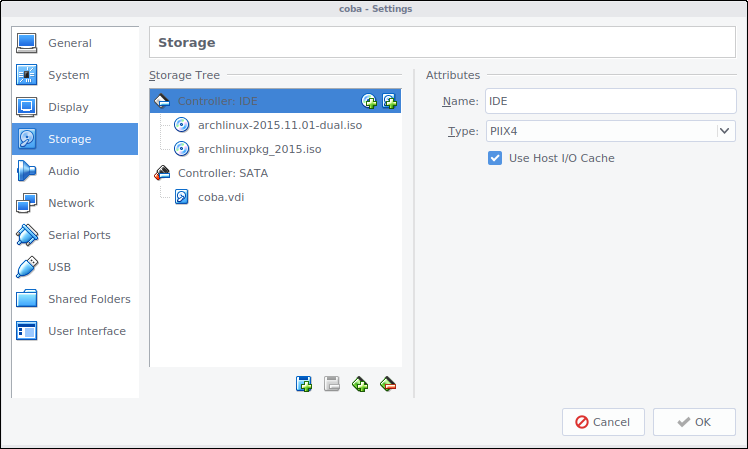
\includegraphics[width=0.4\linewidth]{images/vbox_installinux/s8}
			\caption{siap instalasi}
		\end{figure}		
		File archlinux-2015.11.01-dual.iso dan file-file di dalam archlinuxpkg\_2015.iso sebenarnya dapat di download di internet.
		Namun untuk menghemat waktu, trainer telah sediakan untuk peserta.

		\item Selanjutnya tekan tombol \textbf{OK} dan dilanjutkan \textbf{Start}.
		Setelah masuk tampilan booting, pilih \textbf{Arch Linux x86\_64}.
		Tekan keyboard Enter(\keys{\return}).
		\begin{figure}[H]
			\centering
			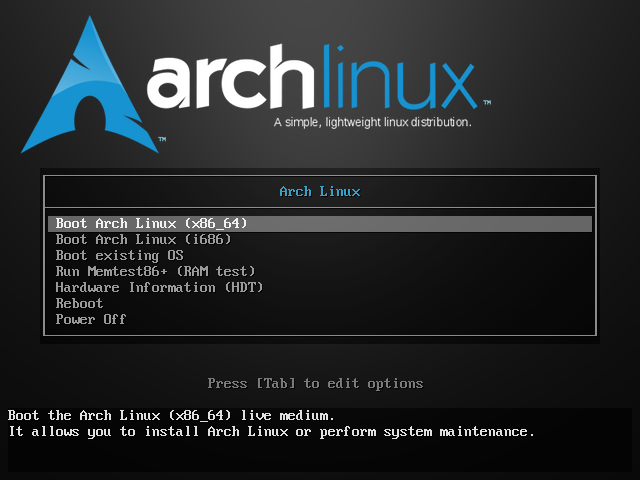
\includegraphics[width=0.4\linewidth]{images/vbox_linuxinstall/s1}
			\caption{Arch Linux x86\_64}
		\end{figure}
	
		\item Tunggu proses booting.
		\begin{figure}[H]
			\centering
			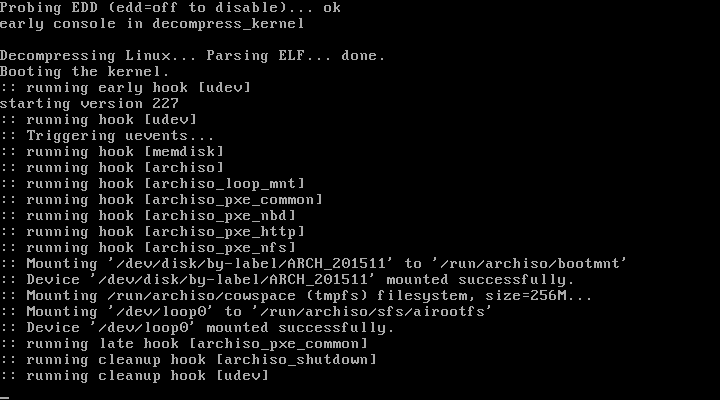
\includegraphics[width=0.4\linewidth]{images/vbox_linuxinstall/s2}
			\caption{mulai booting}
		\end{figure}
	
		\item Booting selesai. Siap instal paket
		\begin{figure}[H]
			\centering
			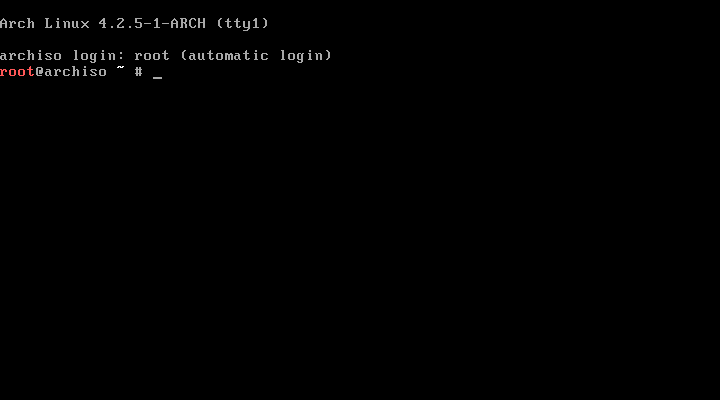
\includegraphics[width=0.4\linewidth]{images/vbox_linuxinstall/s3}
			\caption{Siap Instal}
		\end{figure}
	\end{itemize}
	
	\subsection{Instalasi}
	Praktikum adalah instalasi sistem operasi sendiri.
	Langkah-langkahnya sebagai berikut:
	\subsubsection{Rangkuman Metode}
	Berikut diagram rangkuman metode instalasi yang akan dilakukan:
	\begin{figure}[H]
		\begin{center}
			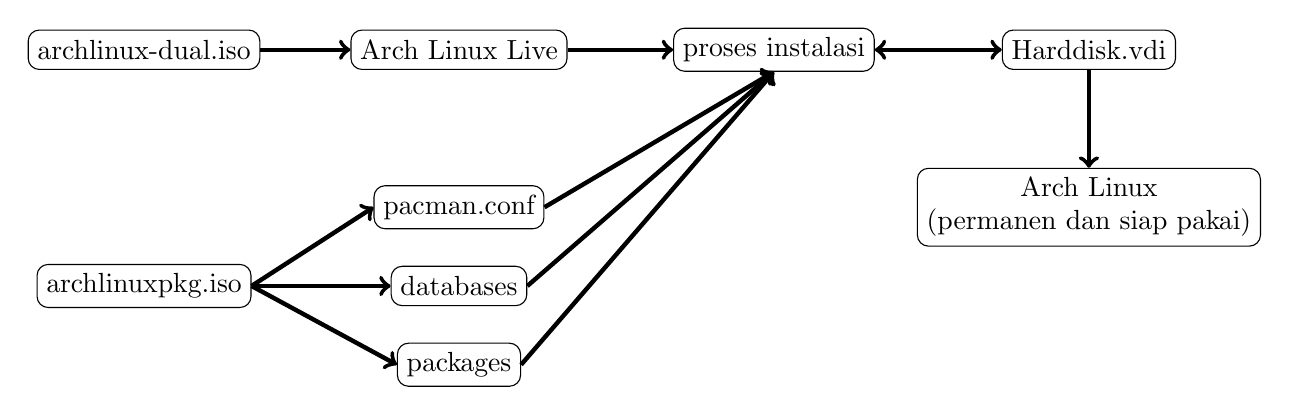
\begin{tikzpicture}[node distance=1cm]
			
			\node (archlive) [squared]  {Arch Linux Live};
			\node (conf) [squared, below of=archlive, yshift=-1cm] {pacman.conf};
			\node (db) [squared, below of=conf] {databases};
			\node (pkg) [squared, below of=db] {packages};			
			\node (archiso) [squared, left of=archlive,xshift=-3cm] {archlinux-dual.iso};
			\node (pkgiso) [squared, left of=db,xshift=-3cm] {archlinuxpkg.iso};			
			\node (install) [squared, right of=archlive,xshift=3cm] {proses instalasi};
			\node (vdi) [squared, right of=install,xshift=3cm] {Harddisk.vdi};			
			\node (archlinux) [squared, below of=vdi,yshift=-1cm,align=center] {Arch Linux\\(permanen dan siap pakai)};
						
			\draw[connect] (archiso.east) -- (archlive.west);
			\draw[connect] (pkgiso.east) -- (conf.west);
			\draw[connect] (pkgiso.east) -- (db.west);
			\draw[connect] (pkgiso.east) -- (pkg.west);
			\draw[connect] (archlive.east) -- (install.west);
			\draw[connect] (conf.east) -- (install.south);
			\draw[connect] (db.east) -- (install.south);
			\draw[connect] (pkg.east) -- (install.south);
			\draw[connect2] (install.east) -- (vdi.west);
			\draw[connect] (vdi.south) -- (archlinux.north);
			
			\end{tikzpicture}
			\caption{Rangkuman Proses Instalasi}
		\end{center}
	\end{figure}	
	
	\subsubsection{Menyiapkan Disk}
	\begin{itemize}
		\item pasang disk kedua (archlinuxpkg\_2015.iso) ke directory \textbf{/mnt}.
		Alamat device \textbf{/dev/sr1} adalah alamat optical disk kedua.
		Perintahnya:
		\begin{minted}[frame=lines,fontsize=\footnotesize]{bash}
mount /dev/sr1 /mnt
ls -l /mnt
		\end{minted}
		
		\item format disk target ke format yang dapat menjalankan Linux/Unix (ext4).
		\textbf{Peringatan:} Hati-hati dalam praktik ini karena bisa menghapus seluruh data.
		Perintahnya:
		\begin{minted}[frame=lines,fontsize=\footnotesize]{bash}
parted /dev/sda mktable msdos
parted /dev/sda mkpart primary 0% 100%
mkfs.ext4 /dev/sda1
		\end{minted}
		
		\item Pasang (\textit{mount}) partisi harddisk \textit{/dev/sda1} ke direktory \textbf{/target}.
		Perintahnya:
		\begin{minted}[frame=lines,fontsize=\footnotesize]{bash}
mkdir -p /target
mount /dev/sda1 /target
ls -l /target
		\end{minted}
	\end{itemize}	

	\subsubsection{Menyiapkan konfigurasi}
	\begin{itemize}
		\item Buat directory konfigurasi paket di \textbf{/target} dan salin konfigurasi dari \textbf{/mnt}.
		Perintahnya:
		\begin{minted}[frame=lines,fontsize=\footnotesize]{bash}
mkdir -p /target/etc/
cp -v /mnt/pacman.conf /target/etc/	
		\end{minted}	
		
		\item Edit skrip instalasi \textbf{/usr/bin/pacstrap} agar cukup mengambil paket yang sudah ada (tanpa mendownload lagi).
		Perintahnya:
		\begin{minted}[frame=lines,fontsize=\footnotesize]{bash}
sed -i "s#-Sy#-S#g" /usr/bin/pacstrap	
		\end{minted}
		
		\item Meng-inisiasi pgp-keyring paket manager. Ini merupakan bagian dari keamanan Arch Linux.
		Perintahnya:
		\begin{minted}[frame=lines,fontsize=\footnotesize]{bash}
pacman-key --init
pacman-key --populate archlinux
		\end{minted}
	\end{itemize}
	
	\subsubsection{Menyalin file-file untuk diinstal}
	\begin{itemize}
	\item Buat directory database di \textbf{/target} dan copy file-file database dari \textbf{/mnt}.
		Perintahnya:
		\begin{minted}[frame=lines,fontsize=\footnotesize]{bash}
mkdir -p /target/var/lib/pacman/sync/
rsync -avh /mnt/databases/ /target/var/lib/pacman/sync/
ls -l /target/var/lib/pacman/sync
		\end{minted}
		
		\item Buat directory cache paket di \textbf{/target} dan copy file-file paket dari \textbf{/mnt}.
		Perintahnya:
		\begin{minted}[frame=lines,fontsize=\footnotesize]{bash}
mkdir -p /target/var/cache/pacman/pkg/
rsync -avh /mnt/packages /target/var/cache/pacman/pkg/
ls -l /target/var/cache/pacman/pkg/
		\end{minted}
	\end{itemize}

	\subsubsection{Memulai instalasi}
	\begin{itemize}
		\item Instalasi paket dasar.
		Berikut paket dasar yang bisa diinstal:
		\begin{itemize}
			\item \textbf{base}. Paket dasar sistem operasi
			\item \textbf{base-devel} dan \textbf{multilib-devel}. Paket dasar untuk kebutuhan kompilasi kode-sumber
			\item \textbf{mkinitcpio}. Paket untuk membangun image kernel dan ramdisk
			\item \textbf{rsync}. Paket untuk synchronisasi konten antar direktory
			\item \textbf{arch-install-scripts}. Paket untuk membantu instalasi Arch Linux lebih lanjut
			\item \textbf{sudo}. Paket untuk membantu menaikkan hak akses
			\item \textbf{grub} dan \textbf{os-prober}. Paket untuk booting sistem operasi
			\item \textbf{virtualbox-guest-utils} dan \textbf{virtualbox-guest-modules-arch}.
			Paket untuk membantu menjalankan sistem operasi dibawah VBox.
			Paket ini tidak dibutuhkan jika instalasi di luar VBox.
		\end{itemize}
		Berikut perintahnya (simbol "\textbackslash" adalah penyambung antar baris):
		\begin{minted}[frame=lines,fontsize=\footnotesize]{bash}
pacstrap -GM -C /target/etc/pacman.conf -d /target \
base base-devel multilib-devel mkinitcpio rsync arch-install-scripts sudo grub os-prober \
virtualbox-guest-utils virtualbox-guest-modules-arch
		\end{minted}
	\end{itemize}

	\subsubsection{Konfigurasi sistem operasi}
	\begin{itemize}
		\item Salin kembali konfigurasi dari \textbf{/mnt} ke root baru.
		Perintahnya:
		\begin{minted}[frame=lines,fontsize=\footnotesize]{bash}
cp -vf /mnt/pacman.conf /target/etc/	
		\end{minted}	
		
		\item \textbf{[Optional]} Edit skrip instalasi \textbf{/usr/bin/pacstrap} di root baru agar cukup mengambil paket yang sudah ada (tanpa mendownload lagi).
		Perintahnya:
		\begin{minted}[frame=lines,fontsize=\footnotesize]{bash}
sed -i "s#-Sy#-S#g" /target/usr/bin/pacstrap	
		\end{minted}
		
		\item Pindah root ke sistem baru.
		Perintahnya:
		\begin{minted}[frame=lines,fontsize=\footnotesize]{bash}
arch-chroot /target
		\end{minted}
		
		\item \textbf{[Optional]} Buat lokalisasi \textit{encoding} bahasa.
		Perintahnya:
		\begin{minted}[frame=lines,fontsize=\footnotesize]{bash}
echo "en_US ISO-8859-1" >> /etc/locale.gen
locale.gen
		\end{minted}
		
		\item \textbf{[Optional]} Buat lokalisasi zona waktu.
		Perintahnya:
		\begin{minted}[frame=lines,fontsize=\footnotesize]{bash}
ln -svf /usr/share/zoneinfo/UTC /etc/localtime
hwclock --systohc --utc
		\end{minted}
		
		\item Atur nama hostname. Gunakan huruf kecil tanpa spasi.
		Disarankan pendek saja.
		Perintahnya:
		\begin{minted}[frame=lines,fontsize=\footnotesize]{bash}
echo "namaanda-PC" > /etc/hostname
		\end{minted}
		
		\item Konfigurasi sistem agar dapat jalan dibawah VBox.
		Jika instalasi bukan di VBox, bisa lompati langkah ini.
		Perintahnya:
		\begin{minted}[frame=lines,fontsize=\footnotesize]{bash}
groupadd -f vboxsf
systemctl enable vboxservice.service
		\end{minted}
		
		\item Tambah username. Gunakan huruf kecil tanpa spasi.
		Nama username harus berbeda dengan hostname.Disarankan pendek saja.
		Perintahnya:
		\begin{minted}[frame=lines,fontsize=\footnotesize]{bash}
useradd -m -g users -G wheel,storage,power,vboxsf,lp -s /bin/bash -c "nama_anda" nama_anda

		\end{minted}
		
		\item Untuk mempermudah pembelajaran, untuk sementara matikan penggunaan password.
		Baik untuk user anda sendiri dan juga root.
		\begin{minted}[frame=lines,fontsize=\footnotesize]{bash}
passwd -d root
passwd -d nama_anda
		\end{minted}
		
		\item Tambah akses superuser anda (melalui program \textbf{sudo}).
		\begin{minted}[frame=lines,fontsize=\footnotesize]{bash}
echo "%wheel ALL=(ALL) NOPASSWD: ALL" >> /etc/sudoers
		\end{minted}
		
		\item Buat tabel partisi disk untuk dijalankan (\textbf{/etc/fstab}).
		Pertama lihat nomor UUID dari disk. Perintahnya:
		\begin{minted}[frame=lines,fontsize=\footnotesize]{bash}
blkid -s UUID -o value /dev/sda1
		\end{minted}
		Masukkan ID disk ke /etc/fstab
		\begin{minted}[frame=lines,fontsize=\footnotesize]{bash}
export MYUUID=$(blkid -s UUID -o value /dev/sda1)
echo "UUID=$MYUUID / ext4 defaults 0 1" > /etc/fstab
		\end{minted}
		
		\item Install ramdisk untuk booting kernel.
		Perintahnya:
		\begin{minted}[frame=lines,fontsize=\footnotesize]{bash}
mkinitcpio -p linux
		\end{minted}
		
		\item Install grub di sistem yang telah terinstal
		Perintahnya:
		\begin{minted}[frame=lines,fontsize=\footnotesize]{bash}
grub-install --recheck --target=i386-pc /dev/sda
grub-mkconfig -o /boot/grub/grub.cfg
		\end{minted}
		
		\item Keluar dari root baru dan matikan komputer VBox
		Perintahnya:
		\begin{minted}[frame=lines,fontsize=\footnotesize]{bash}
exit
shutdown now
		\end{minted}
	
	\end{itemize}
	
	\subsection{Setelah instalasi VBox}
	Selanjutnya adalah konfigurasi Di VBox agar booting dari harddisk yang telah diinstal Arch Linux.
	Langkah-langkahnya:
	\begin{itemize}
		\item Selanjutnya tekan tombol \textbf{Settings}. Pilih tab \textbf{System}.
		Disini ditampilkan urutan media booting.
		Saat instalasi, digunakan \textbf{Optical Disc}.
		Setelah instalasi, maka booting pindah ke Hardisk.
		Gunakan panah disamping daftar media untuk mengganti urutan. 
		\begin{figure}[H]
			\centering
			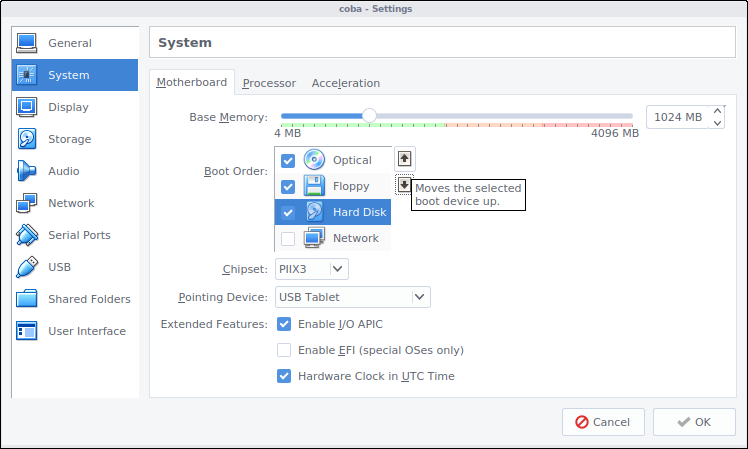
\includegraphics[width=0.4\linewidth]{images/vbox_afterinstall/s1}
			\caption{Atur urutan media instalasi}
		\end{figure}
	
		\item Booting VBox sebagai Harddisk urutan pertama.
		Tekan tombol \textbf{OK} dan dilanjutkan \textbf{Start}.
			\begin{figure}[H]
			\centering
			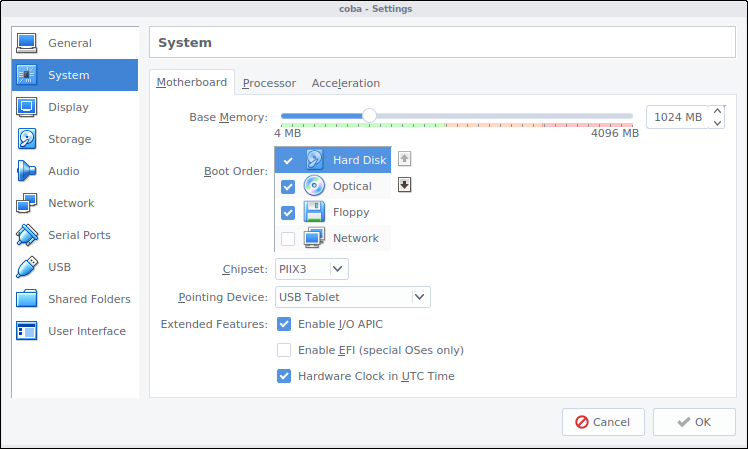
\includegraphics[width=0.4\linewidth]{images/vbox_afterinstall/s2}
			\caption{Booting ke hardisk}
		\end{figure}
	
		\item Selanjutnya tekan \textbf{OK} dan dilanjutkan \textbf{Start}.
		Maka sistem yang telah terinstal tadi akan masuk tampilan pilihan booting (GRUB).
		Jika ada OS lain (semisal Windows atau MacOS), maka akan ada tambahan pilihan untuk booting OS tersebut.
		Pilih \textbf{Arch Linux} dan tekan keyboard Enter(\keys{\return}).
		Tekan keyboard Enter(\keys{\return}).
		\begin{figure}[H]
			\centering
			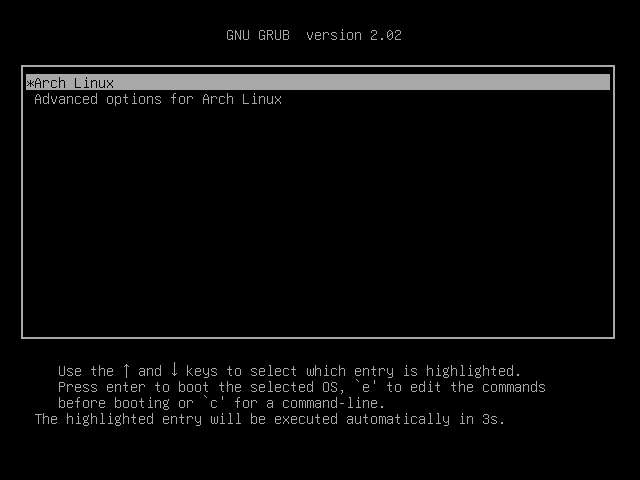
\includegraphics[width=0.4\linewidth]{images/vbox_afterinstall/s3}
			\caption{Tampilan pilihan booting}
		\end{figure}
	
		\item Tunggu beberapa detik untuk proses booting.
		Selanjutnya akan diminta username yang telah dibuat tadi untuk login:
		Ketikkan username nya dan tekan keyboard Enter(\keys{\return}).
		\begin{figure}[H]
			\centering
			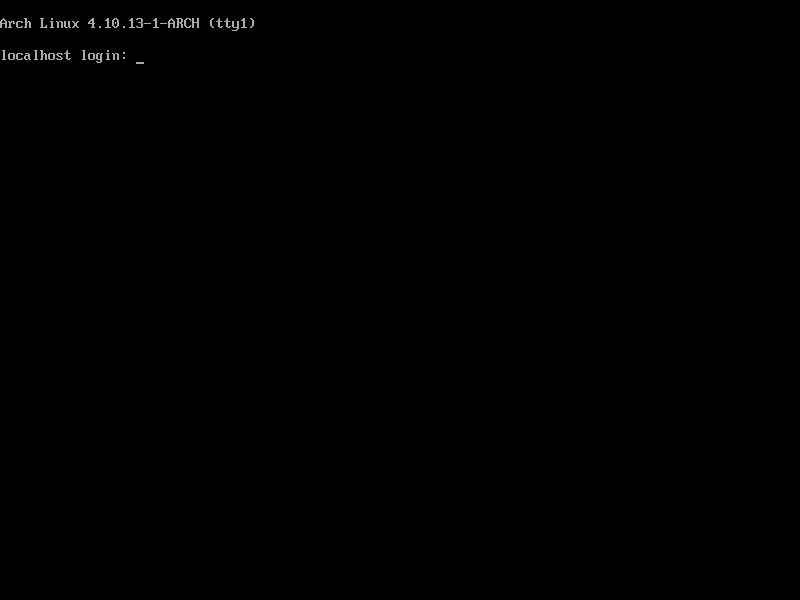
\includegraphics[width=0.4\linewidth]{images/vbox_afterinstall/s4}
			\caption{Tampilan login}
		\end{figure}
	
		\item \textbf{Selamat}, anda sudah berhasil menginstal (membangun) Arch Linux pertama anda.
		\begin{figure}[H]
			\centering
			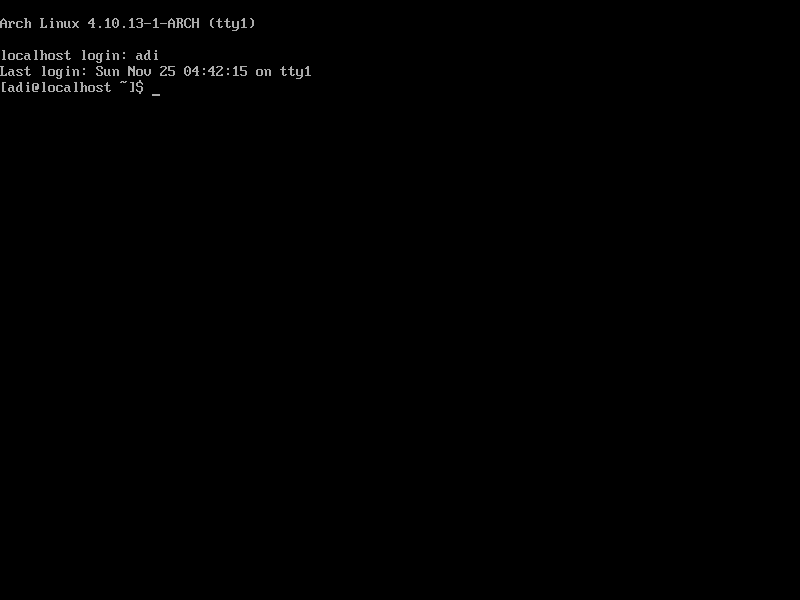
\includegraphics[width=0.4\linewidth]{images/vbox_afterinstall/s5}
			\caption{Arch Linux}
		\end{figure}
	\end{itemize} 

	\subsection{Directory}	
	
	Dalam sistem operasi berbasis UNIX (Linux, BSD, Darwin, MacOS, etc), seluruh directory (folder) dimulai dari alamat "/".
	Anda bisa cek directory ini dengan perintah:
	\begin{minted}[frame=lines,fontsize=\footnotesize]{bash}
ls -l /
	\end{minted}
	\begin{figure}[H]
		\begin{center}
			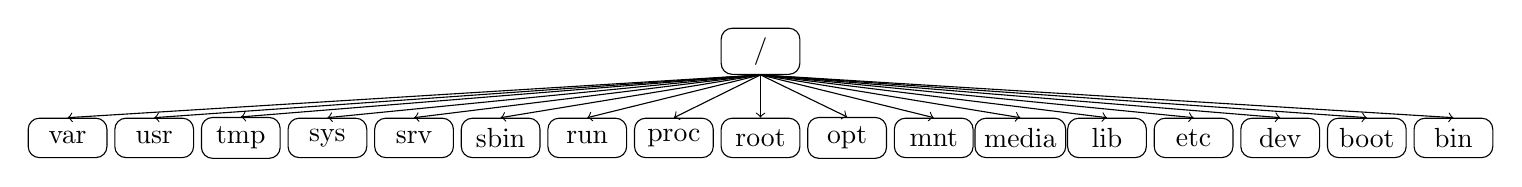
\begin{tikzpicture}[node distance=1.1cm]
			\node (root) [squared] {root};
			
			\node (opt) [squared, right of=root] {opt};
			\node (mnt) [squared, right of=opt] {mnt};
			\node (media) [squared, right of=mnt] {media};
			\node (lib) [squared, right of=media] {lib};
			\node (etc) [squared, right of=lib] {etc};
			\node (dev) [squared, right of=etc] {dev};
			\node (boot) [squared, right of=dev] {boot};
			\node (bin) [squared, right of=boot] {bin};
						
			\node (proc) [squared, left of=root] {proc};
			\node (run) [squared, left of=proc] {run};
			\node (sbin) [squared, left of=run] {sbin};
			\node (srv) [squared, left of=sbin] {srv};
			\node (sys) [squared, left of=srv] {sys};
			\node (tmp) [squared, left of=sys] {tmp};
			\node (usr) [squared, left of=tmp] {usr};
			\node (var) [squared, left of=usr] {var};
			
			\node (path) [squared, above of=root] {/};
			
			\draw[->] (path.south) -- (bin.north);
			\draw[->] (path.south) -- (boot.north);
			\draw[->] (path.south) -- (dev.north);
			\draw[->] (path.south) -- (etc.north);
			\draw[->] (path.south) -- (lib.north);
			\draw[->] (path.south) -- (media.north);
			\draw[->] (path.south) -- (mnt.north);
			\draw[->] (path.south) -- (opt.north);
			\draw[->] (path.south) -- (proc.north);
			\draw[->] (path.south) -- (root.north);
			\draw[->] (path.south) -- (run.north);
			\draw[->] (path.south) -- (sbin.north);
			\draw[->] (path.south) -- (srv.north);
			\draw[->] (path.south) -- (sys.north);
			\draw[->] (path.south) -- (tmp.north);
			\draw[->] (path.south) -- (usr.north);
			\draw[->] (path.south) -- (var.north);
			
			\end{tikzpicture}
			\caption{Hierarki directory UNIX}
		\end{center}
	\end{figure}	

	Berikut penjelasan setiap directory utama:
	\begin{itemize}
		\item \textbf{/}. Directory induk. Dari alamat ini semua alamat absolut direktory utama bermula.
		\item \textbf{/bin}. Directory binary. Disini semua file program yang dijalankan (binary,script,) ditempatkan.
		Khusus Arch Linux, directory /bin adalah \textbf{symlink} dari \textbf{/usr/bin}.
		\item \textbf{/boot}. Directory boot. Disini ditempatkan semua file yang berkaitan dengan booting. Beberapa yang menarik:
		\begin{itemize}
			\item \textbf{/boot/grub/}. GRUB Bootloader.
			\item \textbf{/boot/initramfs-linux.img}. Bagian kernel Linux yang menjadi file system memory (RAM) 
			\item \textbf{/boot/vmlinuz-linux}. Bagian kernel Linux yang diload oleh initramfs ke RAM
		\end{itemize}
		\item \textbf{/dev}. Directory Device. Disini ditempatkan semua file kernel module (driver) dan file-file teks representasi hardware.
		\item \textbf{/etc}. Directory Setting. Disini ditempatkan semua file teks pengaturan global dari sistem operasi. Beberapa yang menarik:
		\begin{itemize}
			\item \textbf{/etc/lightdm}. Pengaturan login desktop LightDM (jika menggunakan).
			\item \textbf{/etc/default}. Berisi beberapa default pengaturan OS.
		\end{itemize}
		\item \textbf{/home}. Diretory user anda. Disini ditempatkan directory user normal (selain super user).
		Disini akan tersedia \textbf{/home/namaanda} tempat menaruh file-file anda.
		\item \textbf{/lib}. Disini ditempatkan semua file pustaka.
		Sebagian besar isi directory \textbf{/bin} membutuhkan file-file pustaka di directory ini.
		Khusus Arch Linux, directory /lib adalah \textbf{symlink} dari \textbf{/usr/lib}.
		\item \textbf{/media}. Directory mounting.
		Disini biasanya sistem operasi otomatis memasang/mengakses media tambahan seperti CD/DVD, USB FD, dst.
		\item \textbf{/mnt}. Directory mounting seperti \textbf{/media}.
		Namun disini tidak ditangani oleh sistem operasi, melainkan bisa oleh pengguna sendiri.
		\item \textbf{/opt}. Directoty Optional.
		Disini biasa ditempatkan software pihak ketiga yang tidak ditangani oleh pengelola paket Arch Linux.
		\item \textbf{/root}. Directory superuser. Fungsinya sebagai home untuk superuser (root).
		Hanya superuser yang memiliki akses ke directory ini.
		\item \textbf{/proc}. Directory proses kernel. Disini ditempatkan semua file yang berkaitan dengan proses kerja kernel.
		\item \textbf{/run}. Directory proses non-kernel.
		Disini ditempatkan semua file yang berkaitan dengan proses kerja program yang sifatnya sementara namun tidak terhapus saat restart.		
		\item \textbf{/sbin}. Directory System Bin. Mirip dengan directory /bin.
		Namun khusus untuk binary yang jalan otomatis seperti program layanan (services).
		\item \textbf{/srv}. Directory Kerja Service. Disini program-program layanan (service) mengambil atau menaruh hasil kerjanya.
		\item \textbf{/sys}. Directory System. Directory ini berisi file-file sistem operasi yang sedang berjalan.
		Directory ini adalah perpanjangan dari directory \textbf{/proc}.
		\item \textbf{/tmp}. Directory Temporary. Berisi file-file hasil kerja program-program yang nanti akan dibersihkan saat restart.
		\item \textbf{/usr}. Directory User system. Berisi file-file bagian sistem operasi yang diinstal oleh pengguna (user).
		Pada banyak sistem operasi Linux, directory ini adalah yang memiliki file terbanyak. Bagian yang menarik:
		\begin{itemize}
			\item \textbf{/usr/bin}. Berisi binary. Untuk Arch Linux, ini adalah directory binary utama
			\item \textbf{/usr/lib}. Berisi library (pustaka). Untuk Arch Linux, ini adalah directory library utama
			\item \textbf{/usr/include}. Berisi pustaka header. Isi directory ini dibutuhkan untuk programming terutama C/C++.
			\item \textbf{/usr/share}. Berisi file-file program resources yang bukan binary dan bukan pula pengaturan.
		\end{itemize}
		\item \textbf{/var}. Directory Variables. Mirip dengan directory \textbf{/tmp}, \textbf{/srv}, atau \textbf{/run},
		namun sifatnya lebih permanen dan sering menjadi directory tembolok (cache).
	\end{itemize}
	
	\subsection{Shell}
	Berikut akan dijelaskan secara mendasar penggunaan antar-muka (\textit{interface}) dari \textit{terminal} atau \textit{shell}.
	\subsubsection{Manajemen Directory/Folder}
	\begin{itemize}
		\item Melihat isi suatu folder.
		\begin{minted}[frame=lines,fontsize=\footnotesize]{bash}
ls [opsi] [alamat_directory]
		\end{minted}
		Berikut beberapa contohnya
		\begin{itemize}
			\item Melihat isi directory \textbf{/usr}.
			\begin{minted}[frame=lines,fontsize=\footnotesize]{bash}
ls /usr
			\end{minted}
			hasilnya:
			\begin{minted}[frame=lines,fontsize=\footnotesize]{text}
arm-none-eabi  examples          lib32    sbin   var
avr            i686-w64-mingw32  lib64    share  x86_64-pc-linux-gnu
bin            include           libexec  src    x86_64-w64-mingw32
etc            lib               local    tests
			\end{minted}
			
			\item Melihat isi directory \textbf{/usr} dalam format daftar (\textit{list})
			\begin{minted}[frame=lines,fontsize=\footnotesize]{bash}
ls -l /usr
			\end{minted}
			hasilnya:
			\begin{minted}[frame=lines,fontsize=\footnotesize]{text}
total 580
drwxr-xr-x   5 root root   4096 May  7  2016 arm-none-eabi
drwxr-xr-x   4 root root   4096 Jul 28  2015 avr
drwxr-xr-x   5 root root 172032 Nov 25 11:22 bin
drwxr-xr-x   3 root root   4096 Mar 20  2016 etc
drwxr-xr-x   2 root root   4096 Jan 19  2017 examples
drwxr-xr-x   5 root root   4096 Nov 21 19:05 i686-w64-mingw32
drwxr-xr-x 551 root root  40960 Nov 24 19:47 include
drwxr-xr-x 303 root root 266240 Nov 24 19:48 lib
drwxr-xr-x  32 root root  36864 Oct  7 20:22 lib32
lrwxrwxrwx   1 root root      3 Mar 27  2017 lib64 -> lib
drwxr-xr-x   3 root root   4096 Oct  7 23:05 libexec
drwxr-xr-x  14 root root   4096 Nov  5  2017 local
lrwxrwxrwx   1 root root      3 Mar 27  2017 sbin -> bin
drwxr-xr-x 371 root root  12288 Nov 24 19:47 share
drwxr-xr-x   3 root root   4096 Oct  7 23:04 src
drwxr-xr-x   6 root root   4096 Jan 19  2017 tests
drwxr-xr-x   3 root root   4096 May  6  2016 var
drwxr-xr-x   3 root root   4096 Oct 31  2016 x86_64-pc-linux-gnu
drwxr-xr-x   5 root root   4096 Nov 21 19:05 x86_64-w64-mingw32
			\end{minted}
			Dalam format list, terdapat informasi tambahan seperti hak akses (\textit{privilage}),
			kepemilikan file (\textit{ownership}),
			ukuran file dalam bytes,
			tanggal/jam terakhir akses/modifikasi,
			dan alamat tujuan jika file tersebut adalah symlink (\textit{symbolic link}).
			
			\item Melihat isi directory sekarang. Jika perintah "ls" tanpa diikuti alamat tertentu, maka directory yang akan ditampilkan adalah directory saat ini
			\begin{minted}[frame=lines,fontsize=\footnotesize]{bash}
ls
			\end{minted}
			hasilnya:
			\begin{minted}[frame=lines,fontsize=\footnotesize]{text}
Arduino       Documents   eagle          PDF        Public          Templates
Desktop       Downloads   IdeaProjects   Pel_Wira   Qucs            Videos
development   ds_sw.ab    Music          Pictures   struktur.dia~  'VirtualBox VMs'
			\end{minted}
			atau apabila dalam format list:
			\begin{minted}[frame=lines,fontsize=\footnotesize]{bash}
ls -l
			\end{minted}
			hasilnya:	
			\begin{minted}[frame=lines,fontsize=\footnotesize]{text}
total 5352
drwxr-xr-x  3 achmadi users    4096 Aug 27 02:10  Arduino
drwxr-xr-x  8 achmadi users   12288 Nov 25 17:58  Desktop
lrwxrwxrwx  1 achmadi users      18 May  6  2016  development -> /home/development/
drwxr-xr-x 23 achmadi users   12288 Nov 18 21:33  Documents
drwxr-xr-x 37 achmadi users   16384 Nov 24 19:48  Downloads
-rw-r-----  1 achmadi users 5385476 Sep 30 23:38  ds_sw.ab
drwxr-xr-x  2 achmadi users    4096 Nov  8 22:15  eagle
drwxr-xr-x  2 achmadi users    4096 Oct 22 20:15  IdeaProjects
drwxr-xr-x  2 achmadi users    4096 Oct  8 10:16  Music
drwxr-xr-x  2 achmadi users    4096 Oct 10 06:12  PDF
drwxr-xr-x  3 achmadi users    4096 Nov 24 21:08  Pel_Wira
drwxr-xr-x  3 achmadi users    4096 Nov 25 11:46  Pictures
drwxr-xr-x  7 achmadi users    4096 Nov 23 12:56  Public
drwxr-xr-x  3 achmadi users    4096 Aug 30 16:24  Qucs
-rw-r--r--  1 achmadi users    1837 Nov 24 14:53  struktur.dia~
drwxr-xr-x  3 achmadi users    4096 Sep 12  2017  Templates
drwxr-xr-x  3 achmadi users    4096 Oct 27 08:00  Videos
drwxr-xr-x  4 achmadi users    4096 Nov 24 16:54 'VirtualBox VMs'
			\end{minted}
			
			\item untuk melihat file/directory yang bersifat hidden, tambahkan opsi -A (\textit{almost all})
			\begin{minted}[frame=lines,fontsize=\footnotesize]{bash}
ls -A
			\end{minted}
			hasilnya:
			\begin{minted}[frame=lines,fontsize=\footnotesize]{text}
total 5352
 .android            .icons                       Public
Arduino             .IdeaIC15                    .python_history
.arduino15          IdeaProjects                 .QtWebEngineProcess
.bash_history       .iprayrc                     .qucs
.bash_logout        .ipython                     Qucs
.bash_profile       .java                        .stm32cubemx
.bashrc             .kchmviewer                  struktur.dia~
.cache              .KiCadLibrarian              .subversion
.cdemu-daemon.log   .klei                        .swt
.config             .local                       Templates
Desktop             .matlab                      .themes
development         .matlab-log                  .thumbnails
.dia               '.Mendeley Desktop'           Videos
Documents           .mozilla                    'VirtualBox VMs'
Downloads           .mtab.fuseiso                .wget-hsts
ds_sw.ab            Music                        .wine
eagle               .nanorc                      .winebcpp
.eagle              .ngspice_history             .winehhc
.eaglerc            .ngspice_history-29825.tmp   .wine-otdr
.eric6              .node_repl_history           .winevc
.esd_auth           .npm                         .wings3d
.FreeCAD            .octave_hist                 .Xauthority
.gimp-2.8           PDF                          .xchm
.gitconfig          Pel_Wira                     .xsession-errors
.gtk-bookmarks      Pictures                     .xsession-errors.old
.ICEauthority       .pki                         .zekr
			\end{minted}
			Tampak lebih banyak file/directory dengan tambahan file/directory yang namanya diawali simbol titik (".").
			Di sistem Unix (Linux, BSD, Darwin, MacOS), untuk membuat file menjadi hidden tinggal tambah titik di awal nama file/directory.
		\end{itemize}
	
		\item Pindah folder/directory.
		\begin{minted}[frame=lines,fontsize=\footnotesize]{bash}
cd [alamat_directory_tujuan]
		\end{minted}
		Berikut beberapa contohnya:
		\begin{itemize}
			\item Sebelum belajar pindah-pindah directory, ada baiknya mengetahui cara mengetahui dimana posisi sekarang.
			Perintahnya:
			\begin{minted}[frame=lines,fontsize=\footnotesize]{bash}
pwd
			\end{minted}
			hasilnya:
			\begin{minted}[frame=lines,fontsize=\footnotesize]{text}
/home/achmadi
			\end{minted}
			
			\item Misal pindah directory \textbf{/usr/bin/}.
			Perintahnya:
			\begin{minted}[frame=lines,fontsize=\footnotesize]{bash}
cd /usr/bin
pwd
			\end{minted}
			hasilnya:
			\begin{minted}[frame=lines,fontsize=\footnotesize]{text}
/usr/bin
			\end{minted}
			
			\item misal pindah satu level di atasnya.
			Perintahnya:
			\begin{minted}[frame=lines,fontsize=\footnotesize]{bash}
cd ..
pwd
			\end{minted}
			hasilnya:
			\begin{minted}[frame=lines,fontsize=\footnotesize]{text}
/usr
			\end{minted}
			Alamat titik dua ("..")	selalu merepresentasikan alamat	satu level di atasnya.
			Anda juga dapat pindah naik lebih dari satu level, misal dengan perintah:
			\begin{minted}[frame=lines,fontsize=\footnotesize]{bash}
cd ../..
pwd
			\end{minted}
			hasilnya:
			\begin{minted}[frame=lines,fontsize=\footnotesize]{text}
/
			\end{minted}	
			
			\item Misal pindah ke folder sendiri.
			\begin{minted}[frame=lines,fontsize=\footnotesize]{bash}
cd /usr/bin
pwd
cd .
pwd
			\end{minted}
			hasilnya:
			\begin{minted}[frame=lines,fontsize=\footnotesize]{text}
/usr/bin
/usr/bin
			\end{minted}
			Alamat titik satu (".") selalu merepresentasikan alamat	folder saat ini.
			
			\item pindah dengan alamat relatif titik satu (".").
			Perintahnya:
			\begin{minted}[frame=lines,fontsize=\footnotesize]{bash}
cd /usr
pwd
cd ./lib
pwd
			\end{minted}
			hasilnya:
			\begin{minted}[frame=lines,fontsize=\footnotesize]{text}
/usr
/usr/lib
			\end{minted}
			Disini perintah kedua tidak perlu mengetikkan alamat lengkat diurut dari root ("/").
			Cukup menggunakan titik (".") sebagai ganti alamat direktory sekarang (\textbf{/usr}).
			
			\item pindah dengan alamat relatif titik satu ("..").
			Perintahnya:
			\begin{minted}[frame=lines,fontsize=\footnotesize]{bash}
cd /usr/bin
pwd
cd ../lib
pwd
			\end{minted}
			hasilnya:
			\begin{minted}[frame=lines,fontsize=\footnotesize]{text}
/usr/bin
/usr/lib
			\end{minted}
			Disini perintah kedua tidak perlu mengetikkan alamat lengkat diurut dari root ("/").
			Cukup menggunakan titik ("..") sebagai ganti alamat direktory sekarang (\textbf{/usr}).
						
		\end{itemize}
	
		\item Membuat Directory
		\begin{minted}[frame=lines,fontsize=\footnotesize]{bash}
mkdir [opsi] [nama_directory]
		\end{minted}
		atau
		\begin{minted}[frame=lines,fontsize=\footnotesize]{bash}
mkdir -p [opsi] [nama_directory]/[nama_directory]
		\end{minted}
		Opsi "-p" untuk membuat direktory beserta \textit{parent}-nya.
		Berikut beberapa contohnya:
		\begin{itemize}
			\item Sebelum belajar membuat/menghapus directory, pastikan anda berada di directory home anda sendiri.
			Mengingat hanya di direktory tersebut anda memiliki hak tulis/baca secara penuh.
			Perintah untuk pindah home:
			\begin{minted}[frame=lines,fontsize=\footnotesize]{bash}
cd ~
			\end{minted}
			Simbol alamat tilde ("\textasciitilde") selalu merepresentasikan alamat home user anda.
			
			\item Membuat direktory dengan nama "coba\_bikin".
			Dilanjutkan perintah melihat isi direktori sekarang.
			Perintahnya:
			\begin{minted}[frame=lines,fontsize=\footnotesize]{bash}
mkdir coba_bikin
ls -l .
			\end{minted}
			\textbf{Catatan:} Hindari nama folder yang memiliki spasi!
			\textbf{Tambahan:} Jika nama folder diawali simbol titik, maka menjadi hidden
			
			\item Membuat direkstory bertingkat.
			Dilanjutkan perintah melihat isi direktori tersebut.
			\begin{minted}[frame=lines,fontsize=\footnotesize]{bash}
mkdir -p coba_bikin/bikin_lagi
ls -l coba_bikin
			\end{minted}
			
			\item Membuat direktory setingkat lebih dari satu.
			Dilanjutkan perintah melihat isi direktori tersebut.
			\begin{minted}[frame=lines,fontsize=\footnotesize]{bash}
mkdir -p coba_bikin/{bikin_lagi,bikin_juga,bikin_kembali}
ls -l coba_bikin
			\end{minted}
		\end{itemize}	
		
		\item Menghapus directory.
		\begin{minted}[frame=lines,fontsize=\footnotesize]{bash}
rm [opsi] [nama_directory]
		\end{minted}
		\begin{itemize}
			\item Berikut contohnya.		
			Dilanjutkan perintah melihat isi direktori sekarang.
			Perintahnya:
			\begin{minted}[frame=lines,fontsize=\footnotesize]{bash}
rm -r coba_bikin
ls -l .
			\end{minted}
			Opsi "-r" berarti menghapus \textit{recursive} yaitu direktori beserta seluruh isinya.
		\end{itemize}
	
		
		\item Menyalin direktory.
		\begin{minted}[frame=lines,fontsize=\footnotesize]{bash}
cp [opsi] [nama_directory] [directory_tujuan]
		\end{minted}
		Berikut contohnya.
		\begin{itemize}
			\item Menyalin satu folder beserta isinya.
			\begin{minted}[frame=lines,fontsize=\footnotesize]{bash}
mkdir coba_baru
mkdir -p coba_bikin/bikin_lagi
cp -r coba_bikin/bikin_lagi coba_baru
ls -l coba_baru
			\end{minted}
		\end{itemize}
					
		\item Mengganti nama direktory.
		Perintah ini juga bisa digunakan untuk memindahkan file.
		\begin{minted}[frame=lines,fontsize=\footnotesize]{bash}
mv [opsi] [nama_directory_lama] [nama_directory_baru]
		\end{minted}
		atau untuk memindahkan
		\begin{minted}[frame=lines,fontsize=\footnotesize]{bash}
mv [opsi] [nama_directory_lama] [nama_directory_tujuan]/[nama_directory_lama]
		\end{minted}
		\begin{itemize}
			\item Berikut contohnya mengganti nama
			\begin{minted}[frame=lines,fontsize=\footnotesize]{bash}
mv -v coba_baru/ baru_coba/
			\end{minted}
			Opsi "-v" berfungsi untuk \textit{verbose} (menampilkan pesan setelah proses berhasil)
			
			\item Contohnya memindahkan
			\begin{minted}[frame=lines,fontsize=\footnotesize]{bash}
mv -v coba_baru/ baru_coba/coba_baru/
			\end{minted}
		\end{itemize}							
				
	\end{itemize}

	\subsubsection{Manajemen File Teks}
	\begin{itemize}
		\item Membuat file teks.
		Perintahnya:
		\begin{minted}[frame=lines,fontsize=\footnotesize]{bash}
touch namafile.txt
ls namafile.txt
		\end{minted}
		
		\item Melihat/Editing isi file teks.
		Terdapat beberapa program untuk melihat isi file teks.
		\begin{itemize}
			\item \textbf{less}. Program less adalah program teks viewer yang popular.
			Perlu diingat bahwa program ini hanya untuk menampilkan isi tanpa bisa edit.
			\begin{minted}[frame=lines,fontsize=\footnotesize]{bash}
less namafile.txt
			\end{minted}	
			Anda dapat menggunakan panah atas (\keys{\arrowkeyup}) dan bawah (\keys{\arrowkeydown}) untuk menggulung tampilan.
			Untuk keluar tekan tombol keyboard huruf \textbf{q}.
			
			\item \textbf{nano}. Program nano adalah program teks editor popular.
			\begin{minted}[frame=lines,fontsize=\footnotesize]{bash}
nano namafile.txt
			\end{minted}
			Anda dapat menggunakan panah atas (\keys{\arrowkeyup}), bawah(\keys{\arrowkeydown}),
			kiri (\keys{\arrowkeyleft}), dan kanan (\keys{\arrowkeyright}) untuk menggulung tampilan.
			Dibawah panel nano terdapat daftar perintah untuk editing.
			Simbol ($\land$) berarti tombol Control (\keys{Ctrl}).
			Perintah umum penggunaan nano:
			\begin{itemize}
				\item Save: \keys{Ctrl} + \keys{o}, dilanjutkan Enter(\keys{\return})
				\item Quit: \keys{Ctrl} + \keys{x}
			\end{itemize}
			
			\begin{figure}[H]
				\centering
				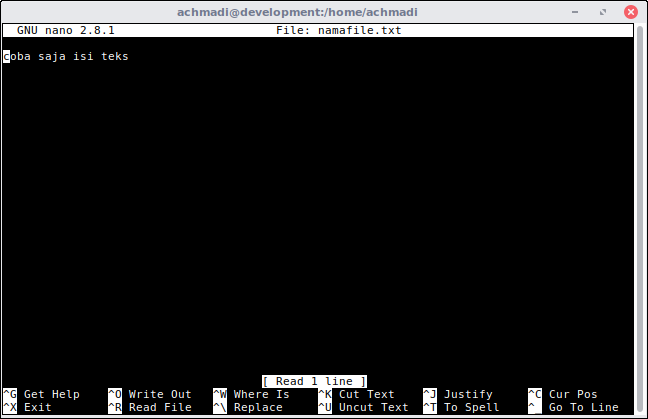
\includegraphics[width=0.4\linewidth]{images/nano}
				\caption{Tampilan editor nano}
			\end{figure}
		\end{itemize}
		
		\item Menyalin file text.
		\begin{minted}[frame=lines,fontsize=\footnotesize]{bash}
cp [opsi] [nama_file] [direktory_tujuan]
		\end{minted}
		Contoh perintah:
		\begin{itemize}
			\item Contoh:
			\begin{minted}[frame=lines,fontsize=\footnotesize]{bash}
mkdir folderbaru
cp -v namafile.txt folderbaru/
			\end{minted}
		\end{itemize}
		
		\item Mengganti nama file text.
		Perintah ini juga bisa digunakan untuk memindahkan file.
		\begin{minted}[frame=lines,fontsize=\footnotesize]{bash}
mv [opsi] [nama_lama] [nama_baru]
		\end{minted}
		atau untuk memindahkan
		\begin{minted}[frame=lines,fontsize=\footnotesize]{bash}
mv [opsi] [nama_lama] [direktory_tujuan]/[nama_lama]
		\end{minted}
		\begin{itemize}
			\item Contoh mengganti nama
			\begin{minted}[frame=lines,fontsize=\footnotesize]{bash}
mv -v namafile.txt namabaru.txt
			\end{minted}
			
			\item contoh dapat untuk memindahkan file
			\begin{minted}[frame=lines,fontsize=\footnotesize]{bash}
mv -v namabaru.txt folderbaru/namabaru.txt
			\end{minted}
		\end{itemize}

		\item Menghapus file.
		\begin{minted}[frame=lines,fontsize=\footnotesize]{bash}
rm [opsi] [nama_file]
		\end{minted}
		\begin{itemize}
			\item Contoh menghapus file
			\begin{minted}[frame=lines,fontsize=\footnotesize]{bash}
rm -v namafile.txt
			\end{minted}
			
			\item Contoh menghapus semua file dalam sebuah direktory
			\begin{minted}[frame=lines,fontsize=\footnotesize]{bash}
rm -v nama_directory/*
			\end{minted}
			Simbol \textit{wildcard} ("*") menjadi pengganti yang bermakna "semuanya".
		\end{itemize}
	\end{itemize}
	
	\newpage
	\section{GUI}
	\subsection{Pengenalan}
	(sedang dikerjakan)
	
	\subsection{Instalasi}
	Praktikum adalah instalasi sistem GUI MATE Desktop.
	Silahkan nyalakan komputer VBox dan login dengan username anda terlebih dahulu.
	Perintah umum instal paket:
	\begin{minted}[frame=lines,fontsize=\footnotesize]{bash}
sudo pacman -S [nama_paket]
	\end{minted}
	Perintah diawali \textbf{sudo} karena untuk instalasi membutuhkan hak superuser.
	Penjelasan lebih detail tentang \textbf{pacman} ada di bab selanjutnya.
	
	\subsubsection{Xorg}
	Pertama instal paket-paket Xorg server terlebih dahulu.
	Xorg disini adalah penyedia (\textit{server}) untuk GUI di shell GNU/Linux.
	Berikut paket-paketnya:
	\begin{itemize}
		\item \textbf{xorg}. Paket ini adalah paket dasar untuk instalasi Xorg server
		\item \textbf{xorg-apps}. Paket ini adalah paket program-program tambahan untuk Xorg server
		\item \textbf{xorg-xinit}. Paket ini adalah paket program inisiasi untuk Xorg server
		\item \textbf{xorg-fonts}. Paket ini adalah paket huruf (\textit{font}) untuk Xorg server
		\item \textbf{xorg-drivers}. Paket ini adalah paket driver display untuk Xorg server
	\end{itemize}
	Perintahnya:
	\begin{minted}[frame=lines,fontsize=\footnotesize]{bash}
sudo pacman -S xorg xorg-apps xorg-xinit xorg-fonts xorg-drivers
	\end{minted}
	
	\subsubsection{LightDM}
	Pertama instal paket LightDM sebagai Login Manager.
	Berikut paket-paketnya:
	\begin{itemize}
		\item \textbf{lightdm}. Paket ini adalah paket dasar untuk LightDM
		\item \textbf{lightdm-gtk-greeter}. Paket ini adalah paket program tampilan LightDM berbasis framework GTK+ 
		\item \textbf{accountsservice}. Paket ini adalah paket pengenalan akun username untuk layanan LightDM
	\end{itemize}
	Perintahnya:
	\begin{minted}[frame=lines,fontsize=\footnotesize]{bash}
sudo pacman -S lightdm lightdm-gtk-greeter accountsservice
	\end{minted}
	
	\subsubsection{Desktop}
	Pertama instal paket MATE Desktop sebagai lingkungan GUI desktop.
	Berikut paket-paketnya:
	\begin{itemize}
		\item \textbf{mate}. Paket ini adalah paket dasar untuk MATE Desktop
		\item \textbf{mate-extra}. Paket ini adalah paket tambahan untuk MATE Desktop
		\item \textbf{ttf-dejavu}. Paket ini adalah paket huruf (\textit{font}) DeJavu
	\end{itemize}
	Perintahnya:
	\begin{minted}[frame=lines,fontsize=\footnotesize]{bash}
sudo pacman -S mate mate-extra ttf-dejavu
	\end{minted}
	
	\subsubsection{Konfigurasi}
	Selanjutnya diperlukan beberapa konfigurasi agar GUI dapat berjalan:
	\begin{itemize}
		\item aktifkan layanan LightDM
		Perintahnya:
		\begin{minted}[frame=lines,fontsize=\footnotesize]{bash}
sudo systemctl enable lightdm
		\end{minted}
		
		\item aktifkan layanan Accounts-Service
		Perintahnya:
		\begin{minted}[frame=lines,fontsize=\footnotesize]{bash}
sudo systemctl enable accounts-daemon
		\end{minted}
	\end{itemize}

	\subsubsection{Login Desktop}
	Selanjutnya anda tinggal reboot/restart dengan perintah:
	\begin{minted}[frame=lines,fontsize=\footnotesize]{bash}
sudo reboot now
	\end{minted}	
	
	Tunggu beberapa saat untuk proses komputer VBox reboot/restart.
	Selanjutnya akan tampil halaman login seperti ini:
	\begin{figure}[H]
		\centering
		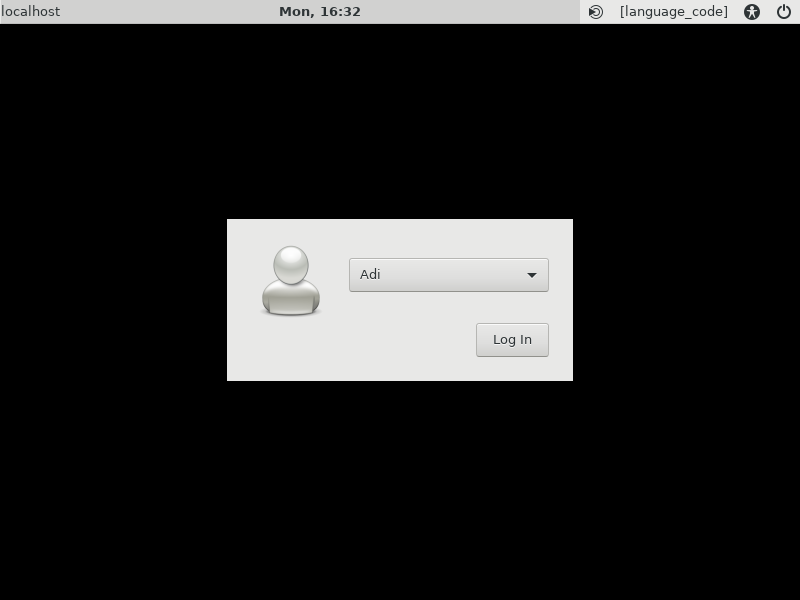
\includegraphics[width=0.4\linewidth]{images/vbox_gui/s1}
		\caption{Tampilan Login LightDM}
	\end{figure}
	Klik tombol \textbf{Log In} pada dialog Login.
	Tunggu beberapa saat, maka akan tampil desktop selayaknya komputer pada umumnya:
	\begin{figure}[H]
		\centering
		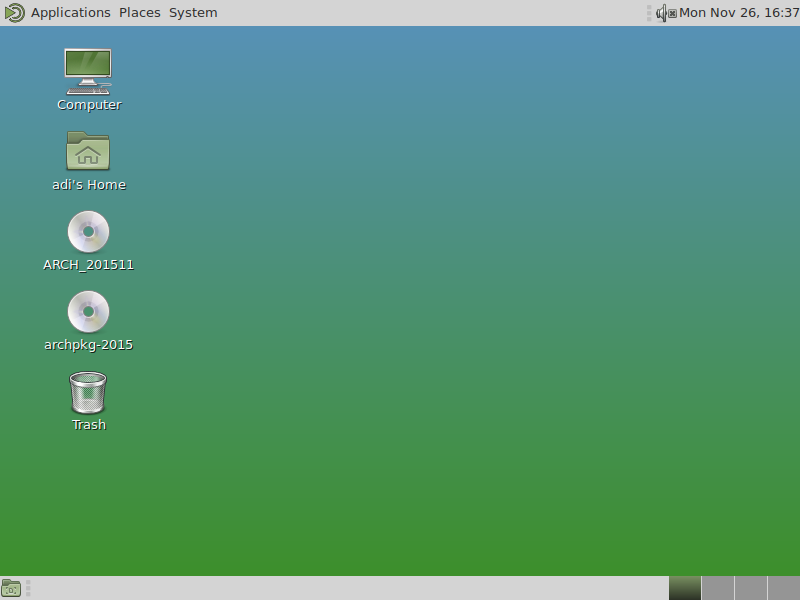
\includegraphics[width=0.4\linewidth]{images/vbox_gui/s2}
		\caption{Desktop MATE}
	\end{figure}
	\textbf{Selamat}. Anda sudah membangun sistem operasi Arch Linux dengan GUI Desktop MATE.
	
	\subsection{Desktop MATE}
	(sedang dikerjakan)

	\newpage
	\section{Pengelola Paket}
	
	\subsection{Pengenalan}
	(sedang dikerjakan)
	
	\subsection{pacman}
	(sedang dikerjakan)

	\subsubsection{install}
	(sedang dikerjakan)
	
	\subsubsection{remove}
	(sedang dikerjakan)
	
	\subsubsection{info: available}
	(sedang dikerjakan)

	\subsubsection{info: installed}
	(sedang dikerjakan)
	
	\subsubsection{info: files}
	(sedang dikerjakan)

	\subsubsection{non-repo}
	(sedang dikerjakan)

	\subsubsection{update}
	(sedang dikerjakan)

	\subsection{makepkg}
	(sedang dikerjakan)
	
	\subsection{alternatif}
	(sedang dikerjakan)
		
	\section{Pemrograman Script Bash}
	
	\subsection{Pengenalan}
	(sedang dikerjakan)
	
	\subsection{Hello World}
	(sedang dikerjakan)
	
	\subsection{Variabel}
	(sedang dikerjakan)
	
	\subsection{Perulangan}
	(sedang dikerjakan)
	
	\subsection{Kondisional}
	(sedang dikerjakan)
	
	\subsection{Argumen}
	(sedang dikerjakan)
	
	\subsection{Fungsi}
	(sedang dikerjakan)
	
	\section{Pemrograman C/C++}
	
	\subsection{Pengenalan}
	(sedang dikerjakan)
	
	\subsection{Hello World}
	(sedang dikerjakan)
	
	\subsection{Makefile}
	(sedang dikerjakan)
	
	\section{Git}
	
	\subsection{Pengenalan}
	(sedang dikerjakan)
	
	\subsection{Instalasi}
	(sedang dikerjakan)
	
	\subsection{status-add-commit}
	(sedang dikerjakan)
	
	\subsection{log-show-tig}
	(sedang dikerjakan)
	
	\subsection{branching}
	
	\section{Wine/Winemaker}
	
	\subsection{Pengenalan}
	(sedang dikerjakan)
	
	\subsection{Instalasi}
	(sedang dikerjakan)
	
	\subsection{Running EXE}
	(sedang dikerjakan)
	
	\subsection{Win32 Programming}
	(sedang dikerjakan)
	
\end{document}
